\documentclass[t]{beamer}
\usetheme{Copenhagen}
\usepackage{amsmath, tikz, bm, pgfplots,cancel}
\pgfplotsset{compat=newest}
\pgfplotsset{every tick label/.append style={font=\scriptsize}}
\setbeamertemplate{headline}{} % remove toc from headers
\beamertemplatenavigationsymbolsempty
\everymath{\displaystyle}
% \usepackage[utf8]{inputenc}

\title{Limits and Algebra}
\author{}
\date{}

\AtBeginSection[]
{
  \begin{frame}
    \frametitle{Objectives}
    \tableofcontents[currentsection]
  \end{frame}
}

\begin{document}

\begin{frame}{}
    \maketitle
\end{frame}




\begin{frame}{Intro}
The graphs of $f(x) = \frac{x^2-6x-7}{x-7}$ and $g(x)=x+1$ are \underline{not the same}.	\newline\\	\pause
\begin{tabular}{p{0.5\textwidth}p{0.5\textwidth}}
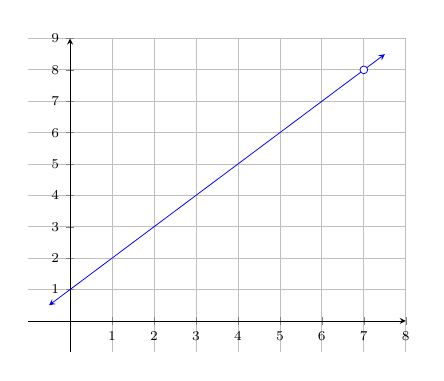
\begin{tikzpicture}[scale=0.7]
\begin{axis}[
	xmin = -1, xmax = 8,
	ymin = -1, ymax = 9,
	axis lines = middle,
	grid,
	xtick = {1,2,...,8},
	ytick = {1,2,...,9}
]
\addplot [<->, >=stealth, domain=-0.5:7.5, color=blue]{x+1};
\addplot [mark = *, color=blue, fill=white] coordinates {(7,8)};
\end{axis}
\end{tikzpicture}
&
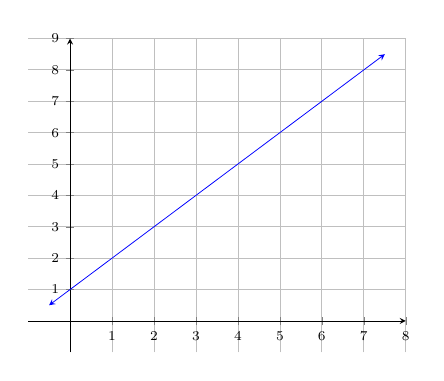
\begin{tikzpicture}[scale=0.7]
\begin{axis}[
	xmin = -1, xmax = 8,
	ymin = -1, ymax = 9,
	axis lines = middle,
	grid,
	xtick = {1,2,...,8},
	ytick = {1,2,...,9}
]
\addplot [<->, >=stealth, domain=-0.5:7.5, color=blue]{x+1};
\end{axis}
\end{tikzpicture}	\\[8pt]
$f(x) = \frac{x^2-6x-7}{x-7}$	&	$g(x)=x+1$	\\
\end{tabular}
\end{frame}

\section{Find Limits via Factoring}

\begin{frame}{Algebraic Limits}
	Some limits that can't be evaluated directly can be evaluated after \alert{cancelling out common factors}.	\newline\\	\pause

	This is called \alert{removable discontinuity}.
\end{frame}

\begin{frame}{Example 1}
	(a) \quad Evaluate $\lim_{x \to -3}\frac{x^2+4x+3}{x+3}$	\newline\\
	\begin{align*}
	\onslide<2->{\lim_{x\to -3} \frac{x^2+4x+3}{x+3} &= \lim_{x \to -3}\frac{(x+3)(x+1)}{x+3}} \\[8pt]
	\onslide<3->{&= \lim_{x\to -3}\frac{\cancel{(x+3)}(x+1)}{\cancel{(x+3)}} } \\[8pt]
	\onslide<4->{&= \lim_{x\to -3} (x+1)} \\[8pt]
	\onslide<5->{&= -3 + 1 } \\[8pt]
	\onslide<6->{&= -2}
	\end{align*}
\end{frame}


\begin{frame}{Example 1}
	(b) \quad Evaluate $\lim_{x\to -2} \frac{x+2}{x^2+7x+10}$	\newline\\
	\begin{align*}
	\onslide<2->{\lim_{x\to -2} \, \frac{x+2}{x^2+7x+10} &= \lim_{x\to -2} \frac{x+2}{(x+2)(x+5)}} \\[8pt]
	\onslide<3->{&= \lim_{x\to -2} \frac{\cancel{x+2}}{\cancel{(x+2)}(x+5)}} \\[8pt]
	\onslide<4->{&= \lim_{x\to -2} \frac{1}{x+5}} \\[8pt]
	\onslide<5->{&= \frac{1}{-2+5}} \\[8pt]
	\onslide<6->{&= \frac{1}{3}}
	\end{align*}
\end{frame}

\section{Limits with Complex Fractions}

\begin{frame}{Complex Fractions}
Simplify the complex fraction by multiplying every term by the \alert{least common tiny denominator}.
\end{frame}

\begin{frame}{Example 2}
Evaluate each.	\newline\\
(a) \quad $\lim_{x\to -5} \left(\frac{\frac{1}{x} + \frac{1}{5}}{x+5}\right)$	\newline\\
\begin{align*}
	\onslide<2->{\lim_{x\to -5} \left(\frac{\frac{1}{x} + \frac{1}{5}}{x+5}\right) &= \lim_{x\to -5} \left(\frac{\frac{1}{x} + \frac{1}{5}}{x+5}\right) \left(\frac{5x}{5x}\right)}	\\[8pt]
	\onslide<3->{&= \lim_{x\to -5} \frac{5+x}{5x(x+5)}} \\
\end{align*}
\end{frame}

\begin{frame}{Example 2}
\begin{align*}
	&= \lim_{x\to -5} \frac{\cancel{5+x}}{5x\cancel{(x+5)}} \\[8pt]
	\onslide<2->{&= \lim_{x\to -5} \frac{1}{5x}} \\[8pt]
	\onslide<3->{&= \frac{1}{5(-5)}} \\[8pt]
	\onslide<4->{&= -\frac{1}{25}} 
\end{align*}
\end{frame}

\begin{frame}{Example 2}
(b) \quad $\lim_{x\to 3} \left(\frac{\frac{1}{3}-\frac{1}{x}}{3-x}\right)$	\newline\\
\begin{align*}
	\onslide<2->{\lim_{x\to 3} \left(\frac{\frac{1}{3}-\frac{1}{x}}{3-x}\right) &= \lim_{x\to 3} \left(\frac{\frac{1}{3}-\frac{1}{x}}{3-x}\right) \left(\frac{3x}{3x}\right)}	\\[8pt]
	\onslide<3->{&= \lim_{x\to 3} \frac{3-x}{3x(x-3)}} \\
\end{align*}
\end{frame}

\begin{frame}{Example 2}
\begin{align*}
	&= \lim_{x\to 3} \frac{\cancel{3-x}}{3x\cancel{(x-3)}} \\[8pt]
	\onslide<2->{&= \lim_{x\to 3} \frac{-1}{3x}} \\[8pt]
	\onslide<3->{&= \frac{-1}{3(3)}} \\[8pt]
	\onslide<4->{&= \frac{-1}{9}}
\end{align*}
\end{frame}

\section{Limits with Radicals}


\end{document}